\documentclass{Phyport}

\usepackage{hyperref}
\hypersetup{
    colorlinks=true,
}

\exname{动态法测量材料杨氏模量} %实验名称
\extable{2}
\instructor{张贯乔} %指导教师
\class{github} %班级
\name{MJ} %姓名
\stuid{2025} %学号

\nyear{2025} %年
\nmonth{11} %月
\nday{17} %日
\nweekday{一} %星期几

\begin{document}
\setcounter{page}{0}
\makecover

\section{预习报告（10分）}
\subsection{实验综述（5分）}

杨氏模量是固体材料在弹性形变范围内正应力与相应正应变的比值，
采用动态弯曲共振法能够较好地测定一些脆性材料的杨氏模量。
 
\begin{figure}[htbp!]
    \centering
    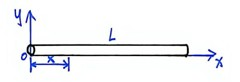
\includegraphics[width=0.3\textwidth]{show.jpg}
\end{figure}

对于一根长度 $L$ 远远大于直径 $d$ 的细棒，$E$ 为杨氏模量，$\rho$ 为材料密度，$S$ 为横截面积，$J$ 为截面惯性矩，
$y$ 为棒上距左端 $x$ 处截面的 $y$ 方向位移，那么作微小弯曲振动时满足动力学方程：
\[
\frac{\partial^4 y}{\partial x^4} + \frac{\rho S}{E J} \cdot \frac{\partial^2 y}{\partial t^2} = 0
\]
边界条件为棒的两端是不受正应力或切向力的自由端。

求解这个方程，在试样作基频振动时，经过处理可以得到杨氏模量为：
\[
E = \frac{1.6067 L^3 m}{d^4} f^2
\]
其中 $L$ 为被测件长度，$m$ 为被测件质量，$f$ 为基频共振频率，$d$ 为圆杆直径。

在实验过程中，由信号源给出等幅正弦波信号经发射换能器转换为机械振动，再传输给被测件上使其受迫作横振动；
接收换能器又将机械振动转变为电信号，经放大处理后显示在示波器上。通过共振频率预估法、峰宽判别法都可以判断试样是否处于最佳共振状态，
这时在频率计上读出信号源的频率即为试样的共振频率，节点处则用外延法推求共振频率，由公式和其他长度、质量的测量量可以计算出试样的杨氏模量。

实验时发现试样在自由状态下被激发产生弯曲振动，振幅在短时间内呈现稳定的周期性变化。观察示波器输出的信号，可以看到当信号源的频率不等于试样固有频率时，
电信号波形很小；而当信号源频率接近试样的固有频率时，电信号突然增大，出现明显的共振峰。

\subsection{实验重点（3分）}

本实验的重点主要在于理解材料在振动状态下的固有频率与其弹性性质之间的关系，掌握动态法测量杨氏模量的基本原理和基本测量方法，
以及了解使用外延法测定试样节点处共振频率的原理和方法。

\subsection{实验难点（2分）}

本实验的难点主要体现在对共振峰的判断上，实际测量时可能会出现多个共振峰，且由于共振峰的幅度受激励强度、拾振位置和环境噪声影响，
某些频率峰值不够尖锐，容易造成判断困难和读数偏差。此外，实验对棒长、质量和截面长度的测量精度要求较高。

\newpage
\section{原始数据（20分）}
实验时记录的数据：
\begin{figure}[htbp!]
    \centering
    
\includegraphics[width=0.75\textwidth]{data.jpg}
\end{figure}

\section{结果与分析（60分）}
\subsection{数据处理与结果（30分）}

\textbf{1.测量材料参数}

用分析天平测量被测件的质量为 $m = 37.437 g$ ，只考虑与仪器有关的 $B$ 类不确定度为 $u_B(m) = \frac{\Delta_{\text{仪}} m}{\sqrt{3}} = 0.6 mg$ 。

分别使用毫米刻度尺和螺旋测微器多次测量被测件的长度和直径并取平均值，其中螺旋测微器的零点误差已经修正：
\begin{table}[htbp!]
    \centering
\begin{tabular}{|l|l|l|l|l|l|l|l|}
    \hline
    次数 & 1 & 2 & 3 & 4 & 5 & 6 & 平均值 \\
    \hline
    $d/mm$ & 5.968 & 5.972 & 5.971 & 5.971 & 5.970 & 5.970 & 5.970 \\
    \hline
    $L/mm$ & 159.6 & 159.7 & 159.8 & 159.7 & 159.9 & 159.9 & 159.8 \\
    \hline
\end{tabular}
\end{table}

计算长度的不确定度时，包括 $A$ 类不确定度：
\[
u_A(L) = \sqrt{\frac{1}{n(n-1)} \sum_{i=1}^{n} (L_i - \bar{L})^2} = 0.05 mm , \quad n = 6
\]
和 $B$ 类不确定度：
\[
u_B(L) = \frac{\Delta_{\text{仪}} L}{\sqrt{3}} = 0.12 mm
\]
总不确定度为：
\[
u(L) = \sqrt{u_A^2 + u_B^2} = 0.13 mm
\]

计算直径的不确定度，同理得到：
\[
u_A(d) = \sqrt{\frac{1}{n(n-1)} \sum_{i=1}^{n} (d_i - \bar{d})^2} = 5.6 \times 10^{-4} mm , \quad n = 6
\]
\[
u_B(d) = \frac{\Delta_{\text{仪}} d}{\sqrt{3}} = 2.3 \times 10^{-3} mm    
\]
总不确定度为：
\[
u(d) = \sqrt{u_A^2 + u_B^2} = 3 \times 10^{-3} mm
\]

\textbf{2.测量共振频率}

\begin{table}[htbp!]
    \left
\begin{tabular}{|l|l|l|l|l|l|l|l|l|l|}
    \hline
    悬挂点到端点的距离 $x / mm$ & 5 & 10 & 15 & 20 & 25 & 30 & 40 & 45 & 50 \\
    \hline
    共振频率 $f / Hz$ & 726.7 & 726.3 & 725.4 & 724.8 & 724.3 & 724.0 & 723.9 & 723.9 & 724.1 \\
    \hline
\end{tabular}
\end{table}

使用MATLAB对测量的共振频率进行二次拟合：
\newpage
\begin{figure}[htbp!]
    \centering
    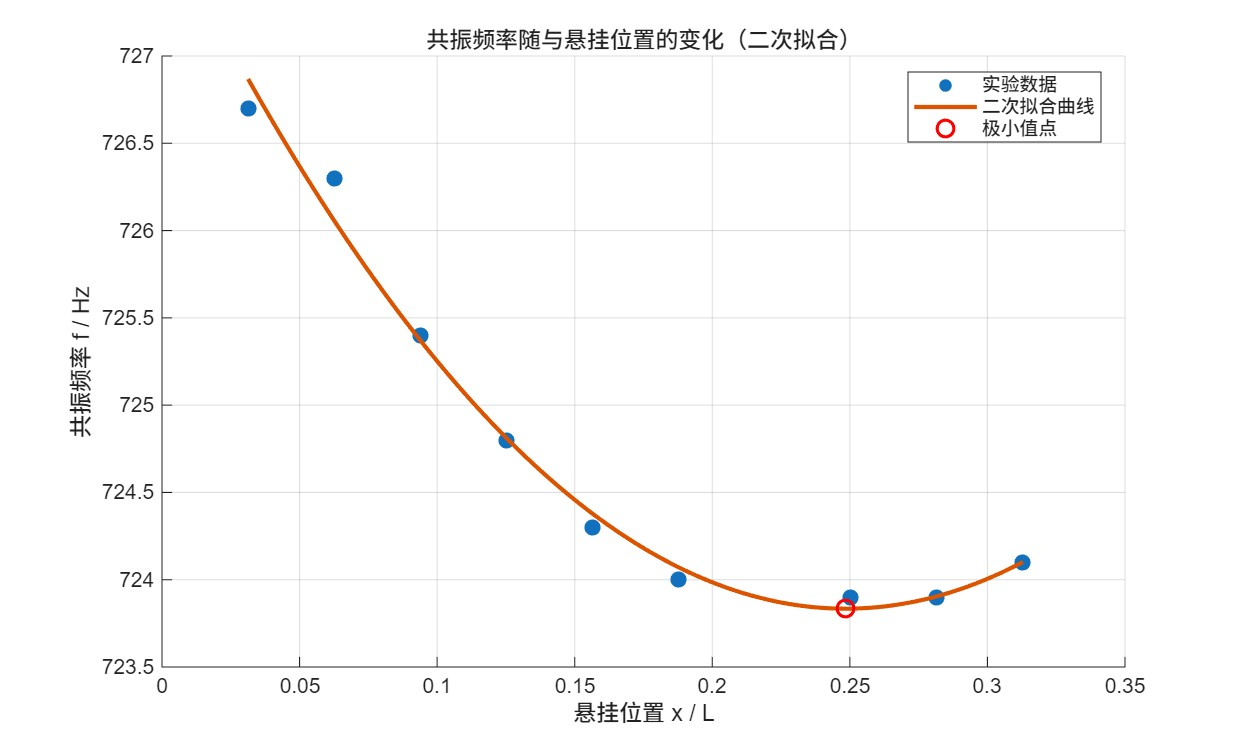
\includegraphics[width=0.6\textwidth]{result.jpg}
\end{figure}
并得出极小值对应频率视为基频共振频率 $f = 723.8 Hz$ ，以三倍频率标准差估计频率不确定度为 $u(f) = 0.34 Hz$ 。

根据杨氏模量计算公式得到：
\[
E = \frac{1.6067 \bar{L}^3 m}{\bar{d}^4} f^2 = 1.016 \times 10^{11} Pa
\]
计算不确定度为：
\[
u(E) = E \cdot \sqrt{(\frac{3 u(L)}{L})^2 + (\frac{4 u(d)}{d})^2 + (\frac{u(m)}{m})^2 + (\frac{2 u(f)}{f})^2} = 3.35 \times 10^8 Pa
\]

最终测量材料的杨氏模量结果为：
\[
E = (1.016 \pm 0.003) \times 10^{11} Pa
\]

\subsection{误差分析（20分）}

查阅资料，铜的杨氏模量约为 $1.1 \times 10^{11} Pa$ ，那么实验测量的相对误差约为 $7 \%$ ，不确定度则相对小，说明存在一定的系统误差，
分析误差来源，主要包括：

1. 使用毫米刻度尺进行长度测量时，用目测的方法对齐示数，导致一定的误差；

2. 测量共振频率时，两根悬线与铜棒的标定悬挂位置很难做到精确对齐，并且悬线不一定完全等长而导致铜棒不完全水平，
都会造成测量误差；

3. 测量共振频率时，示波器显示的信号有微小抖动并且易受外界干扰，难以精确判断峰值，可能会导致误差；

4. 测量时使用的铜棒，可能不是完全的纯铜，或者有氧化、热胀冷缩等的影响，也会导致误差。

\subsection{实验探讨（10分）}

本实验通过动态法测量金属棒的共振频率，从而计算材料的杨氏模量。实验中随着悬挂点位置的改变，
棒的共振频率出现变化，并且在接近杆长中部时出现极小值。通过测量金属棒的质量、长度和直径，
并利用二次拟合和外延法获得基频频率，代入理论公式求得杨氏模量，结果基本合理。

\section{思考题（10分）}

\textbf{1. 如何区分假的共振峰？}

采用共振频率预估法，在实验前先根据理论公式估计共振频率的大致范围，比如本实验以 $725.0 Hz$ 为基础，
然后进行后续频率的细致调节和测量。

采用峰宽判别法，真的共振峰峰宽十分尖锐且稳定，而假的共振峰峰宽较宽、幅度不稳定，
通过改变激振信号频率约 $0.1Hz$ ，就可以判断出被测样是否处于最佳共振状态。

\textbf{2. 测量的实验条件是否满足杆振动模型的要求？}

本实验的条件满足杆振动模型的要求，根据欧拉-伯努利梁理论检查实验条件：
首先，金属棒的长度 $L$ 远大于直径 $d$ ，基本可以忽略剪切与转动惯性的影响；
其次，实验时金属棒的振幅明显小于横截面尺寸，线性应力和应变的关系能够成立；
最后，金属棒质量和几何分布基本均匀，用细线悬挂的方式干扰小，基本满足自由梁的状态。

\textbf{3. 假如不满足，为什么能采用这种方法测出横杆基频？}

这个方法的可行性主要是因为横杆具有明显的基频振动并且稳定性较好：
首先，根据振动理论，固有频率由系统的整体质量分布和弯曲刚度决定，
在边界条件或杆的形状稍微偏离理想模型时，系统仍然存在明显的振动状态和稳定的最低固有频率，基频位置变化不大；
其次，基频对应振动中只有一个弯曲腹，能量集中、振幅极大，在受到激励频率时产生明显响应，并且峰值稳定、不容易被干扰；
最后，根据杨氏模量的实验计算公式，条件偏差造成的误差相对来说非常小，因此测量结果仍然是合理的。

\textbf{4. 我们能否观察 $n=2, 3$ 等情况的本征振动来测量杨氏模量？有什么困难？}

理论上，基频 $n=2, 3$ 等高阶模态也满足欧拉-伯努利振动方程，如果能够测量出对应的频率，就可以计算杨氏模量。

但是，在实际实验中，观测和利用高阶模态具有明显困难。
首先，高阶模态对应的振型结点增多、杆上的振幅分布更加复杂，
而激振位置和拾振器位置有限，如果它们恰好位于结点附近，则信号显著减弱，导致频率难以识别；
其次，高阶模态的能量分布分散、激励效率远低于基频，需要更强激振或更灵敏的检测才能获得清晰谱峰；
再次，高阶模态频率间隔随 $n$ 的增大而变密，谱线容易因环境噪声、仪器带宽或数据处理误差而重叠，增加识别难度；
此外，欧拉-伯努利模型在高频时误差变大，剪切变形和转动惯性无法忽略，导致理论公式与真实频率的差距更明显。

总而言之，虽然观察高阶模态理论可行，但在一般实验条件下，由于识别困难和模型偏差都使其难以用于精确测量杨氏模量，因此本实验采用信噪比最高、模态最清晰的基频模式进行测量。


\begin{thebibliography}{9}
    \bibitem{ref1}
    陈洪叶. 铜棒动态杨氏模量求解方法[J]. 山东农业大学学报（自然科学版）,2010,41(1):125-128. DOI:10.3969/j.issn.1000-2324.2010.01.027. 
    \bibitem{ref2}
    朱华,李翠云. 动态法测金属杨氏模量实验中的谐振频率[J]. 物理实验,2004,24(7):3-5. DOI:10.3969/j.issn.1005-4642.2004.07.001. 
    
    \bibitem{ref3}
    陈洪叶,陈军,韩岳. 动态杨氏模量实验中真假共振信号的分析[J]. 大学物理实验,2017,30(6):22-25. DOI:10.14139/j.cnki.cn22-1228.2017.06.007. 

    \bibitem{ref4}
    刘复乐,祖洪飞,陈章位. 基于金属材料多阶谐振的杨氏模量动态测量方法[J]. 计测技术,2025,45(4):149-157. DOI:10.11823/j.issn.1674-5795.2025.04.11. 

\end{thebibliography}

\input{注意事项}
\end{document}
